\chapter{利用竞价型实例加速大规模计算密集型并行任务}
\label{cha:no2}

\section{本章概述}
\label{sec:no2_intro}
快速发展的云平台向云租户提供了大量充足的计算资源。每个数据中心,每天通常有数千个服务器节点正在处理海量的并行计算任务以支撑大规模的信息检索、数据分析或科学计算等应用。在这样一个大规模的计算架构下,有效且健壮的任务处理框架是非常关键的。这样的计算框架应提供一种可行的方式方便使用者组织和使用底层巨大的计算资源池。具体来说,该计算框架应该能够促进应用开发和部署过程,同时负责调度程序在众多服务器节点上高效运行。近年来已经涌现了许多大规模分布式计算框架,最成功且有代表性的当属 MapReduce \cite{Dean:2004:MSD:1251254.1251264}。

在云平台中,同一台物理机上运行的多台同样配置的虚拟机可能存在显著的性能差异。虽然虚拟化实现了对 CPU 和内存资源的有效隔离,物理机的 I/O 和网络带宽却是由其上的所有虚拟机共享的。这样的共享策略目的在于充分利用物理机的带宽资源,在其它虚拟机不使用 I/O 或 网络资源时可以独占全部带宽,在多个虚拟机竞争 I/O 或网络带宽时均分带宽资源。带宽的竞争可能来自云平台中的其它用户,也可能来自用户自身申请的其它虚拟机。另外,硬件、软件、配置等方面的错误也可能带来一段时间的虚拟机性能下降。再者,虚拟集群内部同时运行的作业之间也可能存在资源竞争。当分布式计算框架使用的虚拟机实例数量达到一定规模时,这类不可预期的节点异常开始变得明显。这些异常者(Outliers)是大规模并行任务处理中最严重的性能杀手。异常者任务的执行进度远远落后于相应的正常任务因而极大地拖延了整个作业的完成时间,进而影响了整个工作流的执行进度。

大规模并行计算任务大体可分为两类:计算密集型任务和数据密集型任务。计算密集型任务在执行的过程中需要大量的CPU时间,性能瓶颈存在于CPU能力上。另一类十分常见的并行处理任务是数据密集型任务,性能瓶颈存在于I/O带宽上。数据密集型任务在执行过程中会产生大量的数据I/O,通常需要处理TB级甚至是PB级的数据,例如:网页索引、数据统计分析等。MapReduce 计算框架主要针对的就是这类数据密集型并行任务。目前在 MapReduce 计算框架上,有很多针对异常者问题的优化工作 \cite{Zaharia:2008:IMP:1855741.1855744, Ananthanarayanan:2010:ROM:1924943.1924962, 180304, Dean:2013:TS:2408776.2408794}。为了解决这一问题,这些优化方法有的依靠任务调度器识别出异常者并通过投机执行策略在其他节点执行同一任务的副本来加速作业执行 \cite{Zaharia:2008:IMP:1855741.1855744, Ananthanarayanan:2010:ROM:1924943.1924962},有的针对集群中的交互式任务 \cite{180304, Dean:2013:TS:2408776.2408794} 采用更激进的克隆任务(Task Cloning)的方法进一步优化响应时间。

MapReduce 等面向数据密集型并行任务的计算框架对异常者的检测基于任务执行进度同输入数据的读取量相一致的假设,通过各个任务的I/O进度识别异常者。显然,这个针对数据密集型并行任务的异常者检测方法并不适合于计算密集型并行任务。而投机执行和任务克隆的方法会消耗大量的计算资源,这对于拥有大量空闲计算资源的本地集群以及只使用少量计算资源的交互式任务来说没有问题,对于部署在云平台上的虚拟集群中的各类大规模并行计算任务则是难以承受的。

本章聚焦于执行 SPMD 任务的分布式处理框架,研究如何利用竞价云计算资源加速大规模计算密集型任务的并行处理。考虑到竞价型实例的易失效特性,将其加入按需型实例组成的虚拟集群做水平扩展是存在问题的。这会让大规模并行计算任务的异常者问题更加严重,将竞价型实例只用做解决异常者问题的额外加速节点显然是更稳妥和巧妙的使用方式。本章设计了一个用竞价型实例来解决云平台中大规模计算密集型并行任务的异常者问题的加速方法,并实现了一个在ProActive计算框架上的原型。针对通过 ProActive 的封装实现并行的大量各类遗留代码(科学计算、工业设计、影像处理渲染等计算密集型应用),该方法使用二进制代码插桩技术实现了对程序执行的跟踪,通过对程序跟踪信息进行聚类分析实现了对异常者的早期发现。通过尽早发现异常者,使用竞价型实例进行低成本的投机执行及任务再分割等策略有效地解决了异常者问题。该加速方法缩短了作业完成时间,提升了云平台中大规模计算密集型并行任务的性能。

总体来说,本章的贡献主要在于:
\begin{enumerate}
\item 在竞价型云平台上设计并实现了一个易于使用、高效低成本的海量计算密集型任务处理框架的任务加速器。
\item 提出了基于二进制代码插桩和聚类分析的大规模计算密集型任务异常者检测方法。该方法在极低的插桩开销下实现了对异常者的早期检测。
\item 使用投机执行、任务再分割任务克隆、等策略有效减少了作业完成时间,基本消除了异常者带来的影响。实验结果表明两个典型的应用 Cap3 和 GaussianBlur 的作业完成时间缩减了超过 20\% 和 40\%,而利用竞价型实例产生的成本开销只有约3\%。
\end{enumerate}

\section{ProActive 框架介绍}
ProActive \cite{ProActive} 并行计算套件是一个开源的应用加速方案。它可以同高性能的云平台管理无缝集成,大大简化了集群并行程序开发。ProActive 的并行分布式计算框架使用Java语言开发,没有对Java虚拟机(Java Virtual Machine)做任何修改。所以 ProActive的扩展性非常好,可以运行在任何支持标准Java环境的操作系统上。利用ProActive,用户可以轻松地加速和编排各种遗留代码应用。

在分布式并行计算环境中,需要一个统一的机制进行作业调度和资源管理。ProActive 使用的是一个批处理式作业调度器 \cite{pascheduling}。该调度器向用户提供了资源的抽象。它允许用户提交包含一个或多个任务的作业,然后在可用的资源上执行这些作业。该作业调度器允许几个用户共享相同的资源池并处理分布式环境下可能出现的问题,如:任务执行失败、资源失效等。该作业调度器也允许用户方便的杀掉一个指定的任务然后在另一个节点上重新执行该任务。

ProActive的作业调度器同资源管理器 \cite{parm} 相连,资源管理器是一个跨网络的资源管理组件。它分配由 ProActive 节点(运行着 ProActive Agent 的 Java 虚拟机)表示的计算资源给作业调度器,作业调度器将可使用的资源分发给各个任务。基于作业调度器、资源管理器和其他组件,ProActive可以无需修改方便地运行在集群、网格、云平台以及各种形式的混合平台上。

\section{系统设计}
\label{sec:no2}
任务加速器主要由两个组件构成:异常者检测和任务执行加速。如图 \ref{figure:no2arch}所示,异常者检测模块通过对任务跟踪信息的分析找出异常者。如果存在异常者,如何利用竞价节点加速任务执行,减少、甚至是消除异常者带来的影响。这是任务执行加速部分的需要解决的问题。通过结合计算复制、投机执行等策略,任务执行加速组件根据异常者情况利用竞价型实例类型的计算资源加速异常者任务的完成,减少异常者带来的影响进而避免整体作业进度的拖慢。
\begin{figure}
  \centering
  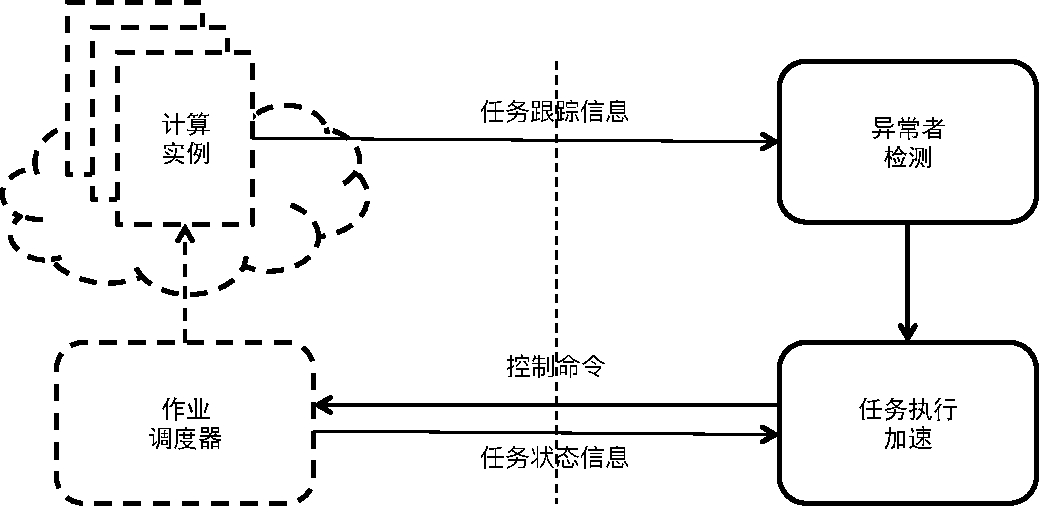
\includegraphics[width=0.8\textwidth]{NO2_arch.pdf}
  \caption{大规模并行任务加速器架构}
  \label{figure:no2arch}
\end{figure}

通过仔细设计接口,整个任务加速器保持了同作业调度器的独立性。这有利于用户根据自身需求选择不同的作业调度器。如图 \ref{figure:no2arch} 所示,任务加速器和 ProActive 作业调度器的接口部分只有获取一个作业的任务状态信息和发送任务管理命令。这些需求可以被任何作业调度器的控制接口满足。

下面将详细介绍系统的两个主要组成部分————异常者检测组件和任务执行加速组件。

\subsection{异常者检测}
\label{subsec:no2_trace}
异常者检测组件通过程序跟踪插桩工具和异常分析两个模块配合实现对大量并发任务中的异常者检测。如图 \ref{figure:tracing}所示,用户只需提供作业程序的二进制代码进行程序跟踪插桩,然后提交XML作业描述文件并使用插桩后的二进制代码作为执行文件。ProActive 作业调度器根据作业描述文件将计算任务分发到各个计算节点,各个节点执行插桩后的程序并返回任务执行进度跟踪信息给异常分析模块。异常分析模块利用聚类分析的手段找出潜在的异常者任务。
\begin{figure}
  \centering
  \includegraphics[width=0.85\textwidth]{NO2_tracing.pdf}
  \caption{程序跟踪插桩}
  \label{figure:tracing}
\end{figure}

异常者检测的实现基于对程序执行的跟踪和对跟踪信息的聚类分析。程序跟踪借助于静态二进制代码插桩实现,在 \ref{subsec:no2_inst} 节详细讨论了需要考虑的问题和主要方法。由于无法根据任务进度跟踪直接得出任务执行进度的准确信息,异常者分析模块的任务就是根据大量任务在执行过程中返回的进度跟踪信息判断是否有潜在异常者存在。在 \ref{subsec:no2_clustering} 节给出了基于机器学习中常用的聚类分析算法的一个简单、有效的发现异常者的方法。

\subsubsection{程序跟踪插桩工具}
\label{subsec:no2_inst}
在实际生产系统中使用二进制代码插桩跟踪程序的执行进度主要有两个挑战。一个挑战是性能开销,即使是轻量级的静态二进制插桩也可能带来数十个百分比的执行时间开销。另一个挑战是如何根据跟踪信息推测执行进度,这里的难点在于:1)在二进制代码中通过插桩工具埋下的程序跟踪点不是完全均匀一致的分布在整个执行过程中的;2)即使程序跟踪点在程序执行过程中均匀的被触发,仍然不能预测出任务已经完成了多少,还要执行多久。

以下载一个文件为例:如果下载进度条一分钟后显示已经完成了 50\%,很明显任务已经完成了一半并且在一个稳定的网络带宽下可能还需一分钟的时间。这就是数据密集型任务的进度预测的基本思路。但对于计算密集型任务来说,二进制程序插桩只能得到程序执行过程中触发了哪些插桩点的信息,无法得知程序执行的绝对进度。没有了类似数据密集型任务输入输出与执行进度相关的假设,计算密集型任务的执行进度很难通过二进制代码插桩进行预测。二进制代码插桩只能作为提供程序执行跟踪信息的手段,而实际上大量并发任务的异常者检测也不必非要预测任务的绝对执行进度。因此程序插桩工具只负责进行程序跟踪,异常者则交由异常者分析模块根据大量并发任务执行的跟踪信息分析得出。在本节我们重点讨论如何解决二进制代码插桩给程序执行带来的性能问题。

通过对多个计算密集型程序的二进制代码插桩和观察,可以得出两个发现:1)程序中不同的函数处在不同的调用层次;2)相同层次的函数被调用的频率相近,少数底层的函数被调用的极为频繁占用了大多数执行时间。表\ref{table:inst-stats}给出了插桩了全部函数入口点的 ImageMagick 动态链接库的函数调用次数统计信息。该函数库中有超过 1060 个函数,其中只有 33 个函数在多次执行中被调用超过 10000 次。
\begin{table}
\centering
\begin{threeparttable}
\caption{ImageMagick 函数调用信息统计}
\label{table:inst-stats}
\begin{tabular}{c|c|c}
\hline
调用次数 & 函数个数 & 函数举例 \\
\hline
above $10^7$ & 6 & CopyMagickMemory \\
$10^6$ - $10^7$ & 16 & GetCacheNexus \\
$10^5$ - $10^6$ & 2 & LocaleCompare \\
$10^4$ - $10^5$ & 9 & GetNexus \\
$10^3$ - $10^4$ & 10 & AddValueToSplayTree \\
$10^2$ - $10^3$ & 17 & FormatMagickStringList \\
$10^1$ - $10^2$ & 78 & NewSplayTree \\
$0$    - $10^1$ & 922 & GaussianBlurImage \\
\hline
\end{tabular}
\small 注:每个调用次数量级只给出一个函数作为例子。 
\end{threeparttable}
\end{table}

函数进入/退出点,和基本块(Basic Block)是常用的二进制代码的程序插桩点。理想的程序执行跟踪是对所有这些插桩点进行插桩,以实现更好的代码覆盖效果。然而,二进制代码程序插桩的开销明显是和埋下的插桩点数量成比例的。通过选择相对粗力度的插桩可以跳过少部分底层函数,从而去掉了大部分的插桩开销。为了能够准确跟踪程序执行,二进制代码的插桩需要足够的覆盖程度。如何在保证足够大范围的插桩覆盖的要求下达到最低的插桩开销?下面给出了基于函数调用次数统计的程序跟踪插桩方法。整个程序跟踪插桩的核心有两点:1)跟踪插桩点的选择;2)插桩点触发时执行的操作。

插桩点选择方法首先对二进制代码中的所有函数埋下插桩点,纪录每个函数的调用情况。然后多次执行插桩后的程序并统计函数调用次数信息。通过多次执行,不同调用层次的函数被区分开来。所有函数被调用次数的均值可以作为一个判断函数是否属于被频繁调用的底层函数的标准。所有大于这个均值的调用次数的函数,在最终的用于跟踪程序执行进度的插桩点选择中得以跳过。对于编程良好的程序,这样的自动插桩点选择方法可以同时保证足够大的执行进度跟踪覆盖和足够低的运行时开销。

在每个选定的程序插桩点可以插入一段代码,这段代码就是插桩点触发时需要执行的操作。对于程序执行的跟踪,在所有选定的函数入口进行插桩可以纪录下该函数调用的相关信息。由于这里程序跟踪的最终目标是在大量并发任务中检测潜在的异常者,在插桩点执行的操作可以简化为将一个插桩点计数器加一。这样就保证了在每个插桩点只有极低的运行开销。

\subsubsection{异常者分析}
\label{subsec:no2_clustering}
对于计算密集型并行任务的加速来说,第一个首要的目标是找出异常者。进行二进制插桩后的程序在各个节点执行,大量的并行任务运行中会提供程序的跟踪信息给异常者分析模块。虽然没有任务执行的绝对进度信息,通过比较所有并行任务的跟踪信息还是可以对潜在的异常者加以区分。这里使用统计分析和数据挖掘中常用的聚类分析方法对各个节点返回的程序跟踪信息进行聚类。对于大规模并行任务节点的程序跟踪信息的聚类分析基于如下假设:
\begin{itemize}
\item 在海量并行任务中,异常者只占较少的一部分。
\item 作业的分割基本保持均匀,即所有任务的规模大致相同。
\item 集群中的服务器节点异常以非确定的方式出现且过一段时间可能恢复正常。
\end{itemize}

异常者由于这样或者那样的原因执行缓慢,在程序跟踪的信息上同正常节点会表现出明显的(甚至是数量级上的)差距。这里使用大规模并行任务进度跟踪反馈的插桩点计数器信息提取每个任务的两个特征作为聚类依据,使用 K-means 聚类分析算法对正常节点和异常者加以区分。这两个特征分别是插桩点计数器累积值和最近一个程序跟踪信息反馈周期的插桩点计数器增量。它们基本反映了任务执行的进度和即时状态。图 \ref{figure:clusteringexample} 给出了一个基于这两个特征进行二类聚类分析的例子。
\begin{figure}
  \centering
  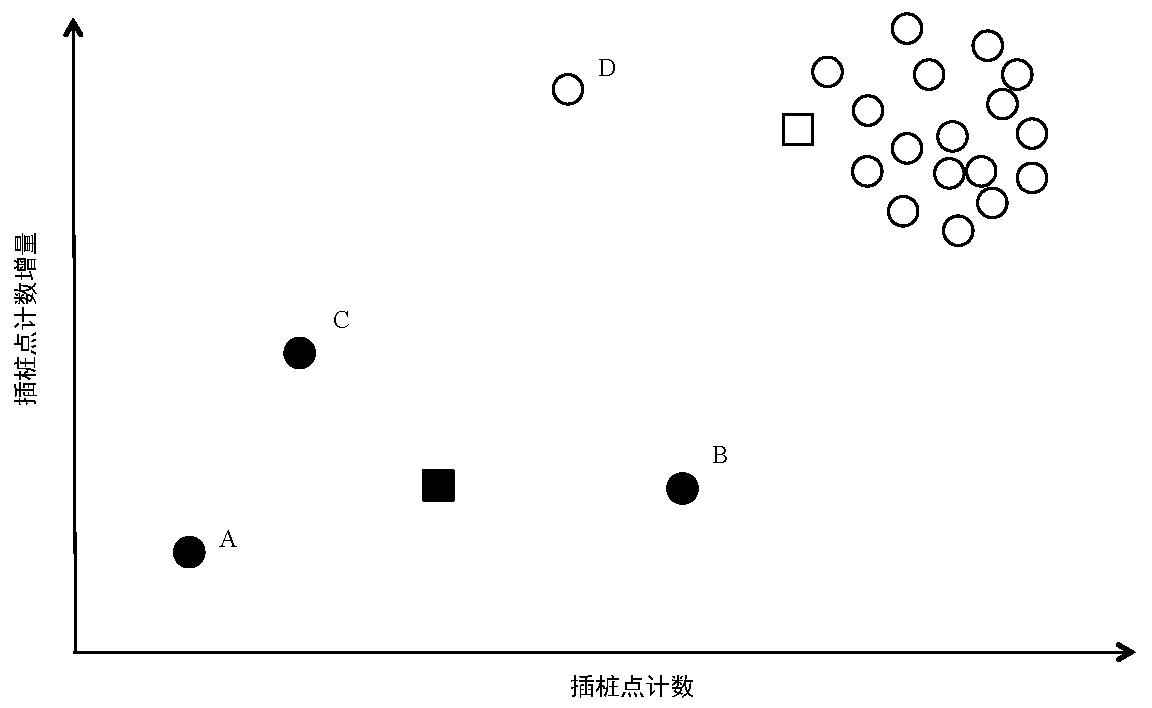
\includegraphics[width=0.8\textwidth]{clusteringexample.pdf}
  \caption{一个对并行任务程序跟踪信息使用K-means进行二类聚类分析的例子}
  \label{figure:clusteringexample}
\end{figure}

程序跟踪信息中插桩点计数器的值可用于在大量并发任务中比较相对的快慢,而最近一个反馈周期的插桩点计数增量体现的则是最近一小段时间某个任务的执行状态。单纯的使用插桩点计数器的值无法快速发现在任务执行过程中出现异常的节点,结合这两个参数可以在把握大量并发任务整体执行状态的同时迅速的找出可疑的异常者。如图 \ref{figure:clusteringexample} 所示,一个简单的 $k = 2$ 的 K-means 聚类可以大致将代表任务执行状态的点分为两类。从图 \ref{figure:clusteringexample} 中显然可以判断出,左下方的 $A$ 点和 $C$ 点极有可能代表异常者的任务状态。对于图 \ref{figure:clusteringexample} 中的 $B$ 点和 $D$ 点,只能认为它们有可能是异常者。对于异常者任务执行加速的目标来说,可以接受误报(False Positive),但不能接受漏报(False Negtive)。因为误报只会损失一些计算资源,而漏报则会直接贻误任务执行加速的时机进而影响作业完成时间。所以,在计算资源允许的情况下合理的策略是对所有潜在的异常者都通过备份执行实现容错。

\begin{algorithm}
\caption{异常者聚类}
\label{fig-outlier-algo}
\KwIn{$traces$}
\KwOut{$outliers$}%
$clusters\gets kmeans(traces, 2)$\;
$outliers\gets[]$\;
\If{$\left|clusters[1].centroid - clusters[2].centroid\right| \gg 0$}
{
  \uIf{$clusters[1].size \ll clusters[2].size$}
  {
    $outliers\gets [clusters[1], outlierClustering(clusters[2])]$
  }
  \ElseIf{$clusters[1].size \gg clusters[2].size$}
  {
    $outliers\gets [clusters[2], outlierClustering(clusters[1])]$
  }
}
\Return{$outliers$}
\end{algorithm}

算法 \ref{fig-outlier-algo} 给出了一个基于 K-means 聚类分析的异常者聚类方法。由于 K-means 算法对初值的选取比较敏感,而这里聚类的目标是将异常者任务和正常任务分成两类。因此可以用所有点中两个特征值的最小值作为一类初始聚类中心,所有点中两个特征值的最大值作为另一类初始聚类中心。如前文所述,异常者检测的目标是报告可疑的异常者。为了减少漏报,可以接受一定程度的误报。因此,在第一次 K-means 聚类后,可以对被认为不是异常者的一类再进行一次同样的 $k = 2$ 的 K-means 聚类分析,以过滤掉图 \ref{figure:clusteringexample} 中的类似 $D$ 点的情形。这样可以保证很大程度上的不漏报。

\subsection{任务执行加速}
在异常者检测组件给出了潜在异常者的情况下,可以利用竞价型实例低成本的执行一个和潜在异常者同样的任务。这样通过对同一个计算任务的投机执行,减轻了某个节点上可能的异常拖慢整体作业执行进度的程度。由于竞价型实例的申请和启动需要几分钟甚至十几分钟的时间,在发现潜在的异常者后再去申请竞价型实例显然就丧失了加速执行的机会。因此系统中需要维护一个竞价型实例资源池,这样在需要对计算任务增加一个执行副本时可以将竞价型实例立即投入使用。大规模并行计算任务运行在按需型实例组成的虚拟集群中,竞价型实例资源池负责提供需要投机执行时的计算资源。所有竞价型实例的竞价设定为市场价格,当市场价格升高实例被回收时则重新申请。如果竞价型实例市场价格超过了相应按需型实例的价格,则没有必要再使用竞价型实例计算资源加速按需型实例上的大规模并行计算任务。

\subsubsection{执行加速策略}
在某个节点可能存在异常的情况下,将其上执行的相同任务在其他节点冗余执行以期容错的机制这里称之为投机执行。当多个执行副本中的一个完成任务时,即可停止其他副本的执行。利用投机执行加速大规模并行任务在策略上有一些直观的经验规则:
\begin{enumerate}
\item 对进度最慢的异常者分配最高的投机执行优先级,显然这是加速作业完成的最优选择。
\item 尽早对潜在异常者发起投机执行。投机执行的目标是尽量减少作业完成时间,尽早执行意味着更好的提早完成的机会。
\item 针对某个异常者任务投机执行时,由于比其它任务开始的晚,为了加快执行速度在任务特点允许的情况下可以将该任务分成若干个子任务交由多个节点执行。
\end{enumerate}

当用户提交作业后,任务执行加速器作为一个守护进程运行在管理节点上。守护进程获取各个任务的程序跟踪信息的频率应该保证不影响ProActive作业管理器的正常执行。任务加速执行策略的主要部分如算法 \ref{fig-acc-algo} 所示,该算法定期的获取各个节点上执行的任务的程序跟踪反馈信息,通过聚类分析找出其中潜在的异常者。对于可能是异常者的任务,使用执行加速策略。对于投机执行的任务,一旦有一个任务副本执行完成,即可停止另一个副本的执行。如果该任务可进行拆分,算法 \ref{fig-acc-algo} 默认将任务拆分为两个子任务执行,在整个作业中已经有任务完成时将任务拆分为更多的子任务以减少任务完成所需时间。当然这要考虑作业的实际情况,在条件允许的情况下进行拆分。
\begin{algorithm}
\caption{执行加速}
\label{fig-acc-algo}
\KwIn{$job$ and sleep $interval$}
\KwOut{$job.state$}
$shards\gets 2$\;
\While{$job.state\not=FinishedOrFaulty$}
{
  \If{$job.finished\_tasks\not=nil$}
  {
    $shards\gets job.finsished\_tasks.size + 1$\;
  }
  $tasks\gets job.unfinished\_tasks$\;
  $outliers\gets outlierClustering(tasks.traces)$\;
  \ForEach{$outlier \in outliers$}
  {
    \If{$! outlier.task.replicated$}
    {
      \eIf{$outlier.task.divisible$}
      {
        $shards\gets min(shards, outlier.task.pieces)$\;
        $r\gets job\_submit(task\_split(outlier.task, shards))$\;
      }{
        $r\gets job\_submit(outlier.task)$\;
      }
      $replications\gets [replications, r]$\;
    }
  }
  $sleep(interval)$\;
  $job.update()$\;
  \For{$r \in replications$}
  {
    \uIf{$r.state = Finished$}
    {
      $kill(r.outlier.taskid)$\;
    }
    \ElseIf{$r.outlier.state = Finished$}
    {
      $kill(r.jobid)$\;
    }
  }
}
\KwRet{$job.state$};
\end{algorithm}

\subsubsection{计算资源利用率优化}
在发现潜在异常者后,除了使用竞价型实例进行针对性的双副本执行,还可以利用系统中空闲的按需型实例进行这样的冗余计算。这种情况可能出现在该节点已经执行完被分配的任务,但整个作业还没有完成的情况。联系算法 \ref{fig-acc-algo},随着部分节点完成任务后开始增加副本执行的任务拆分个数就是基于这一点考虑。

在用户提交作业后向各个节点分发任务前,由于还没有潜在异常者的出现竞价型实例将处于空闲状态。这部分空闲的计算资源也可以用来进行纯粹的``复制执行'',即在不知道各个节点状态的情况下冗余执行一些任务的副本。由于竞价型实例资源池一般小于按需计算实例的规模,因此投机执行只能针对部分节点。一个简单的策略是选择上次作业执行过程中出现的异常者节点,如果还有剩余的竞价型实例则可以随机指定。在作业开始执行后出现异常者时,如果恰好有对应的备份执行节点且正常则不用再投机执行该任务。如果没有对应的备份执行节点,可以停掉某个两个任务备份都正常执行的双副本中的竞价型实例上的任务副本用于提供给新出现的异常者做任务投机执行。

\section{系统实现}
\label{subsec:no2_impl}
为了更好的理解,本节对大规模计算密集型并行任务加速器中一些重要的实现细节加以解释。原型系统中使用的技术和一些背后的实现技巧也进行了简短地介绍。

二进制插桩部分基于DynInst \cite{Dyninst-Deconstruction} 插桩库的静态插桩实现。DynInst 是一个支持对二进制代码进行静态插桩,或对运行中的进程进行动态插桩的工具函数库。它提供了一个机器无关的构建插桩工具和应用的接口。插桩点选择部分对所有函数调用次数的统计基于DynInst的一个使用例程,CodeCoverage \cite{codecoverage}。
	
对于插桩点选择器,有三个代码片段(Code Snippet)插桩到程序中:初始化部分代码片段插桩到程序的开始,用于创建一些数据结构用于统计所需信息;最为常用的代码片段插桩到所有函数的入口点,用于纪录每一次函数调用;最后一个代码片段插桩到程序的结束,用于将函数统计信息保存到一个文件。同样有三个代码片段用于最终的任务进度跟踪插桩,初始化和结束部分用于申请和释放共享内存。最常用的代码片段负责将程序跟踪插桩计数加一。

任务加速器的投机执行部分基于 ProActive Scheduler \cite{pascheduling} 实现。通过控制脚本,任务加速器可以同ProActive的作业调度器进行交互。控制脚本是Javascript风格的语言,解释引擎基于集成于Java SE发行版的 Rhino \cite{Rhino:2016} 脚本引擎。通过控制脚本可以在运行时调用Java实现的ProActive作业调度器的对象和方法。

任务加速器根据异常者聚类结果选择需要进行投机执行的任务。对于每个异常者,生成一个紧急作业并给予一个根据异常者拖慢进度的程度确定的优先级。每个紧急作业可能包含一个或多个需要执行的任务,所有这些紧急作业按照投机优先级顺序提交给作业调度器。通过在作业描述中声明执行节点选择并提供节点选择脚本可以避免投机执行的任务被再次提交到一个异常节点。可以根据任务的大小选择调整异常者检测和执行加速的间隔,避免过于频繁的交互对作业调度器造成的干扰。程序跟踪信息只有插桩点的计数,所占用的内存和传输带宽非常小,对性能的影响可以忽略不计。

在整个实现中还提供了三个Shell脚本用于任务分割,本地代码封装,以及结果合并。Shell脚本将被提交给作业调度器作为正常作业执行。这实例上类似 MapReduce 任务的处理方式。用户只需增加具体的任务切分的命令到任务分割脚本中和一个收集结果的命令到结果合并脚本中,这对于一些作业可能是不必要的。一些默认的步骤,如:拷贝分割后的输入文件到任务执行节点,也可以根据具体情况进行修改。在本地代码封装脚本中,本地程序通过一条命令执行。用于传输任务跟踪信息的守护进程也在这个脚本中启动。用户可以极为灵活的使本地程序得以大规模并行。

为了更好的程序执行性能,程序的插桩部分使用共享内存将结果传递给传输任务进度跟踪信息的守护进程,通过对内存的读写实现了纪录程序跟踪数据的目的。这样每次程序执行过程中遇到插桩点时只引入了内存写操作,相对文件读写大大降低了性能开销。

\section{系统评测}
\label{sec:no2_eval}
通过一系列在云平台中展开的实验,本节给出了大规模计算密集型并行任务加速器的性能相关的评测结果。系统原型部署在 Amazon EC2 云平台的 ``us-east1'' 区域,使用 StarCluster \cite{starcluster} 将虚拟机计算实例组织成一个虚拟集群。StarCluster \cite{starcluster} 是一个 Amazon EC2 云平台上自动化虚拟集群构建、配置、管理的工具包,可以简化整个虚拟集群的部署过程。在虚拟集群中一个 EBS 被挂载在 Master 节点作为共享存储上以 NFS 文件系统的方式共享给集群中的所有节点。ProActive Scheduler 和本章的任务加速器部署在虚拟集群的 Master 节点上,虚拟集群中的虚拟机实例被以 SSH 架构类型节点资源的形式纳入到 ProActive 框架的管理调度中。虚拟集群中的计算资源包括 200 个按需型实例,以及在同一可用区维护的竞价型实例计算资源池。虚拟集群中所有虚拟机实例的配置类型选用 ``linux.m1.small'' 类型节点。该类型实例有 1.7 GB 内存和一个虚拟 CPU 核(约一个 EC2 运算单元的计算能力),存储块设备为 EBS。

实验中选用的代表性应用有两个:一个是生物信息学领域的 Cap3 \cite{Huang:1999:Cap3},另一个是影像处理中常用的 ImageMagick \cite{imagemagick}。Cap3 是生物信息学中比较常见的基因序列拼接组装程序,它的输入是许多FASTA格式 \cite{fasta} 的表达序列标签(Expressed Sequence Tag)文件。Cap3作业接受的输入是一些需要尝试进行序列拼接的FASTA文件,每个Cap3任务处理这样的一个或若干个文件。另一个应用 ImageMagick 是经典的开源影像处理工具,被广泛用于图像处理渲染等。其中的高斯模糊(Gaussian Blur)是一个常用的图像处理手段,在数学上看高斯模糊就是图像与正态分布(高斯分布)做卷积。高斯模糊能够减少图像中的噪点以及降低层次细节,常用于计算机视觉算法中的预先处理阶段,也被称为高斯平滑。实验中使用 Gaussian Blur 作为另一个应用案例,一个 Gaussian Blur 作业需要对大量的图片进行高斯模糊处理,每个任务需要处理一张或多张这样的图片。

评测中的第一个测试是针对程序跟踪带来的插桩性能开销的微基准测试,这关系到本章的任务执行加速器是否能用于实际的生产系统中。云平台的异常者情况也通过实验数据加以验证。系统评测中最主要的指标是作业完成时间,它直接反映出任务加速和性能提升的效果。另外,系统的计算资源使用率和一个长期的成本开销也是需要考虑的方面。

\subsection{程序插桩开销}
\label{sec:no2_overhead}
在任务加速器中,程序跟踪是异常者检测的基础。静态二进制代码插桩相比动态插桩的运行时开销已经小了很多,但如果对所有函数入口都埋入插桩点跟踪程序进度仍有不小的开销。这将使得任务加速器在异常者问题上的优化大打折扣甚至毫无意义。基于对程序执行过程中函数调用层次的观察,这里使用了一种基于采样的插桩点选择方法,在保证覆盖绝大多数函数的同时过滤掉了极少数调用频率特别高的函数,大大减少了程序跟踪插桩带来的开销。微基准测试集中对两个程序 Cap3 和 ImageMagick 使用两种不同的插桩方式得到的二进制代码在同一节点上执行,没有插桩的原始二进制代码作为基线也在相同节点上执行了同一任务。不同二进制代码的执行时间如图 \ref{figure:inst_overhead} 所示,插桩全部函数入口点在两个程序的执行中约带来 10\% 左右的运行时开销,而系统中使用的基于采样的程序跟踪插桩几乎和原始二进制代码执行时间相同,增加的运行时开销约0.1\%。

\begin{figure}
  \centering
  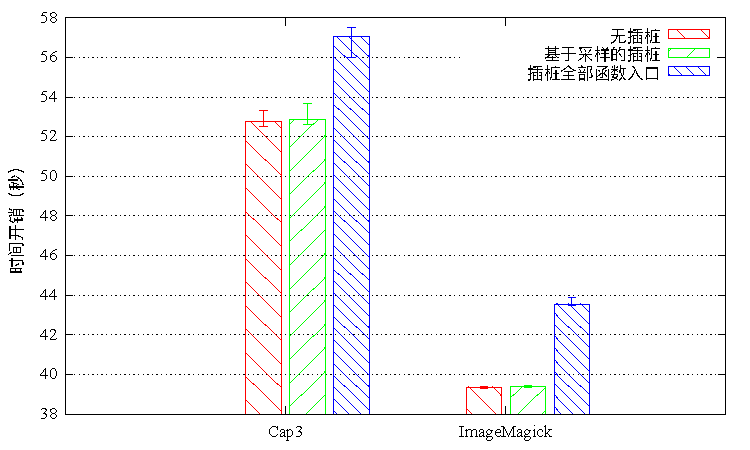
\includegraphics[width=0.9\textwidth]{inst_overhead.pdf}
  \caption{程序跟踪的插桩开销}
  \label{figure:inst_overhead}
\end{figure}

实验结果显示本系统使用的基于采样的程序跟踪插桩开销足够小,对程序的执行性能没有明显影响,可以用于大规模实际生产系统中。

\subsection{异常者情况}
云平台中异常者的现象在一个大规模虚拟集群中非常普遍,有些时候相对正常节点在I/O、网络性能上有明显下降。在其上运行的程序可能受到严重影响。为了测试虚拟集群中的异常者,这里向 ProActive 框架提交一个有100个相同任务的Cap3作业。在一天内不同阶段多次重复这个实验,可以发现异常者的情况有所区别,但很多时间段内都存在少量的明显慢于其它节点任务执行速度的节点存在。这里给出其中异常者较为严重的一次测试结果,具体如图 \ref{figure:outlier_cloud} 所示。
\begin{figure}
  \centering
  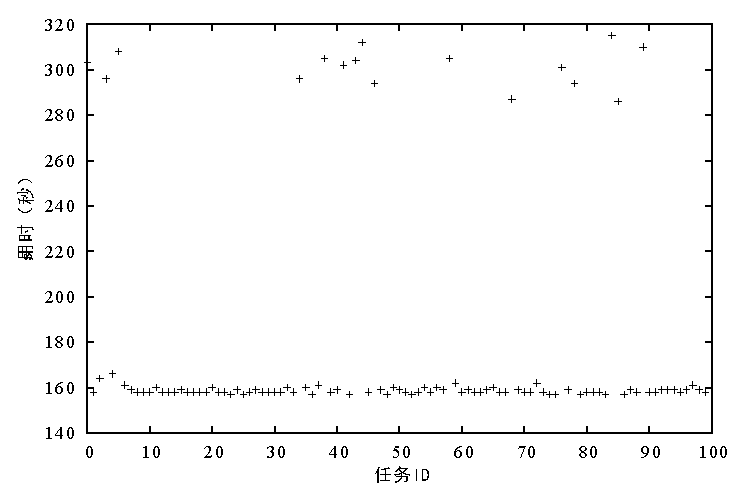
\includegraphics[width=0.8\textwidth]{cloud_outliers.eps}
  \caption{Amazon EC2云平台中100个节点在一次运行Cap3作业时的任务完成时间}
  \label{figure:outlier_cloud}
\end{figure}

从图 \ref{figure:outlier_cloud} 中可以看出,异常者可能导致整个作业被拖慢两倍甚至更长的时间。当虚拟集群中节点数量可观时出现异常者的情况变得常见。一个针对大规模并行任务集群的日志统计结果 \cite{Ananthanarayanan:2010:ROM:1924943.1924962} 显示有 25\% 的作业中有超过 15\% 的异常者出现。对于大规模并行计算任务来说,考虑异常者对整体作业进度的影响十分必要。

\subsection{性能改进}
\label{sec:no2_perf}
性能测试使用了虚拟集群中的200个按需计算实例,利用竞价型实例作为执行加速的廉价计算资源。在实验过程中,通过向 ProActive Scheduler 提交包含 200 个任务的 Cap3 作业或 GaussianBlur 作业测试了在不使用本章提出的任务加速器、使用本章任务加速器但不使用初始阶段的任务克隆策略,以及同时使用投机执行策略和任务克隆策略三种系统配置下的作业处理性能。测试中所使用的作业任务规模大小接近:Cap3 任务为对一个FASTA格式文件中的基因序列进行拼接,不可继续进行分割;GaussianBlur 任务为对一张图片进行高斯模糊处理,根据实际计算中的近似算法可继续分割。

竞价型实例计算资源池中的节点数量可以综合考虑成本因素,以及短期内异常者出现比率设定。用于消除异常者影响的竞价型实例数量不足可能导致有异常者没有对应的执行副本,最终仍拖慢作业完成进度。因此,在性能测试中首先要确定的是竞价型实例计算资源池中所需的节点数量。在一段时间内,针对两个应用分别尝试提供占所有按需型实例数量(本实验中为200个)不同百分比的竞价型实例数用于投机执行,在这个测试中不引入完成自身任务的空闲按需型实例进行投机执行。测得的作业完成时间如图 \ref{figure:replica_cap} 所示,在 Cap3 作业中有 9\%(18个)的竞价型实例用于投机执行就很好的抑制了异常者造成的影响,在 Gaussian 作业中则需要至少 24 个节点用于投机执行才起到减少作业完成时间的效果。这是因为 GaussianBlur 任务可以进行再次拆分,每次投机执行都会使用更多的计算节点。在用于投机执行的节点数达到 18\% 之后基本起到了消除异常者的效果,GaussianBlur 作业通过对任务拆分加快了任务执行进一步减少了作业完成时间,从而得到了比 Cap3 作业更好的性能提升。根据上述测试结果,接下来的性能测试中在竞价型实例资源池中维护 18\%(36个)的计算资源。为保证测试数据的准确性,在一段时间内相同的实验被重复多次,最后的结果取平均值和最小、最大值。实验结果如图 \ref{figure:completiontime_cloud} 所示。
\begin{figure}
  \centering
  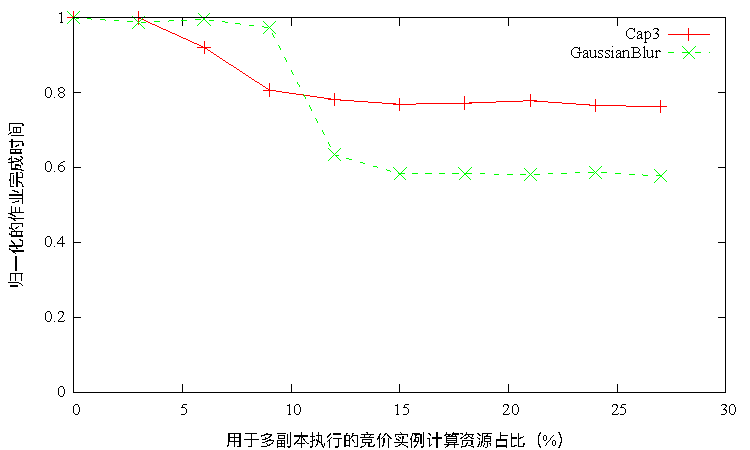
\includegraphics[width=0.9\textwidth]{replica_cap.pdf}
  \caption{用于投机执行的竞价型实例数同作业完成时间的关系}
  \label{figure:replica_cap}
\end{figure}

作业完成时间完全由执行最慢的任务决定。从图 \ref{figure:completiontime_cloud} 中可以看出,实验中作为基线的不使用任务加速器的 ProActive 框架的平均作业完成时间远远大于最好情况下的作业完成时间,这说明在大规模并行任务执行中异常者对整体作业执行带来的拖慢影响十分严重。在使用了投机执行策略后,Cap3 作业的平均完成时间被有效缩减了超过 20\%。由于 Cap3 任务不可继续分割,投机执行策略无法通过再次分割任务的方式加快任务执行。实验结果上看,在投机执行策略下 Cap3 作业的平均完成时间同没有异常者的最好情况仍有一段差距。因为,在发现异常者时副本执行的任务已经落后于正常节点。GaussianBlur 作业的平均执行时间在使用投机执行策略后将作业完成时间缩减了超过 40\%,接近作业执行时间的最好情况,基本消除了异常者带来的影响。这是因为虽然发现异常者时已经落后于正常节点,GaussianBlur 任务可以通过进一步分割减少完成任务所需的时间。如图 \ref{figure:completiontime_cloud} 所示,在任务初始阶段的任务克隆策略只在 Cap3 作业执行中带来了少量的性能提升,对于 GaussianBlur 作业则没有明显效果。虽然任务初始阶段的投机执行有潜在的性能优化机会,但由于异常者出现的不确定和偶发性其所能带来的性能提升在实验中并不明显。在任务不可分割的情况下,能一定程度上进一步减少异常者造成的拖慢作业完成时间影响。
\begin{figure}
  \centering
  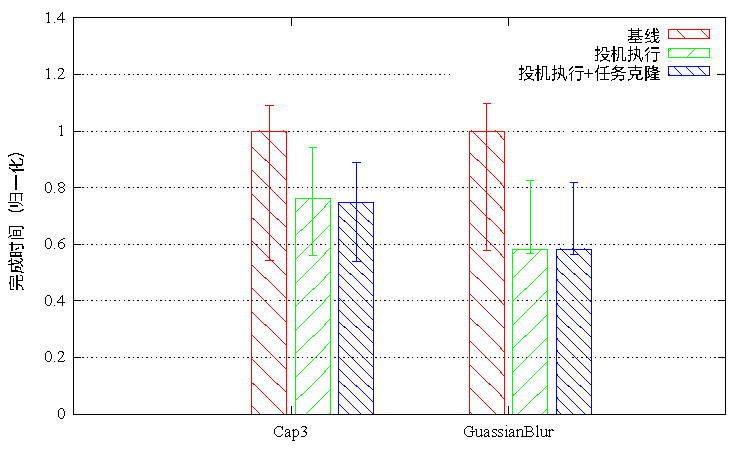
\includegraphics[width=0.9\textwidth]{cloud_completiontime.pdf}
  \caption{虚拟集群中的ProActive作业完成时间比较}
  \label{figure:completiontime_cloud}
\end{figure}

\subsection{资源使用率与成本开销}
\label{sec:no2_usage}
在进行性能测试的同时,ProActive Resource Manager 统计的CPU使用率也能一定程度上反映作业执行的效率。如图 \ref{figure:resourceusage_cloud} 所示,在大规模并行任务执行过程中,异常者不仅拖慢了整体作业完成进度还造成了一定的计算资源的空闲和浪费。在两个作业的执行中,均只有不到 50\% 左右的CPU使用率。使用投机执行和初始阶段任务克隆的策略,加快了作业完成进度,减少了计算资源的空闲时间。在任务可再次分割的情况下,更是能够充分利用已经完成任务执行的空闲节点计算资源。投机执行策略使 Cap3 作业的执行中 CPU 使用率增加到了约 70\%,在 Gaussian 作业中CPU使用率更是接近 90\%。
\begin{figure}
  \centering
  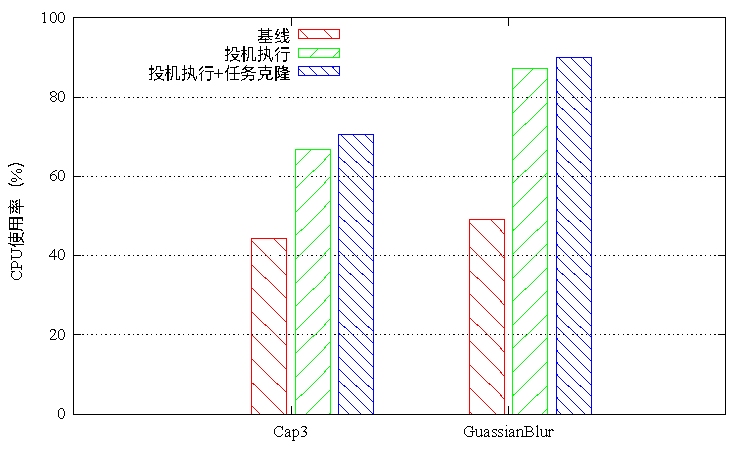
\includegraphics[width=0.9\textwidth]{cloud_usage.pdf}
  \caption{虚拟集群在ProActive作业执行中的CPU使用率比较}
  \label{figure:resourceusage_cloud}
\end{figure}

在计算成本开销方面,从长期的 Amazon EC2 云平台竞价型实例市场价格的历史数据看,竞价型实例的成本约为相同类型的按需成本的五分之一到十分之一。以本实验中使用的``linux.m1.small'' 类型来说,对于一个有200个按需计算实例的虚拟集群来说,36个竞价型实例的计算成本只有虚拟集群成本的约 3\%。

\section{本章讨论}
本章详细介绍了利用竞价型实例加速大规模计算密集型并行任务的方法,基于程序跟踪和聚类分析等手段实现了对海量并发计算密集型任务中的异常者的早期检测,通过投机执行等策略实现了作业完成时间的缩减,消除了异常者造成的影响。该方法的有效性在系统评测中得到了验证,但在实际应用中仍有一些需要注意的地方。

\subsection{对竞价节点的使用}
本章提出的大规模计算密集型并行任务处理加速方法,解决的是云平台虚拟集群中偶发性的节点异常拖慢作业完成进而影响工作流进度的问题。需要强调的是对竞价型实例的使用,本章的工作中将竞价型实例只用于投机执行等加速策略因而隔离了竞价节点失效对系统可靠性的影响。简单地将虚拟集群中的按需型实例全部或者部分换成同样成本但数量更多的竞价型实例似乎能进一步提升系统并发能力,实则不可行。云平台异常者的产生多种多样,包括:硬件故障、软件配置错误、共享I/O和网络带宽资源导致的竞争等。竞价节点潜在的不可靠性引入了一种新的节点异常,但这类异常完全不同于其它:1)竞价节点失效不是性能变差而是直接停机;2)竞价节点的异常不是偶发性、少量的,大量同一可用区竞价型实例的失效是强相关的。这同本章介绍的任务加速方法假设的系统中的异常者只占很少一部分相违背。而针对大量的节点异常使用投机执行策略时,大量新的执行副本同样面临执行过程中的异常者问题。事实上,这是另一个问题,即:在使用竞价型实例执行计算任务时如何处理竞价不足的节点失效问题。

\subsection{成本收益分析}
对于本章要解决的问题,一个十分简单的处理方法是更加激进的使用复制执行策略。在全部任务开始执行的时候直接进行冗余执行,每个任务有两个副本来消除异常者带来的影响。相对带来的性能提升,无论是使用按需型实例还是竞价型实例作为执行副本的计算资源都是不划算的。再考虑异常者长期的出现频率,使用一定比例的按需型实例作为执行副本的计算资源仍是一个很高的成本。相对应的,极为低廉的价格以及作为备用执行副本不要求可靠性的用途让竞价型实例成为了加速异常者的最佳选择。

\section{本章小节}
同以往的工作不同,本章提出了利用竞价型实例解决大规模计算密集型并行任务的异常者拖慢作业进度的低成本方法。该方法的原型实现在 ProActive 框架上,引入了针对大规模计算密集型任务的异常者检测方法。该方法通过组合基于二进制插桩的程序跟踪技术和基于聚类分析的异常者分析方法实现了对异常者的早期发现。在程序跟踪方面,通过基于采样的插桩点选择方法在保证足够覆盖性的前提下将插桩的运行时开销从 10\% 降低到了 约 0.1\%。投机执行和任务克隆等策略一定程度上消除了异常者的影响,针对任务可继续分割的情况通过使用多个节点完成一个异常者任务加速进一步减少了作业完成时间。针对两个典型应用的评测结果显示本章的工作实现了对大规模计算密集型任务的加速,大大减轻了异常者的影响。作业完成时间的缩减在两个应用中分别超过 20\% 和 40\%,而计算成本的增加只有约 3\%。